The goal of this chapter is to show the results of the algorithms for MCE-$k$ and MCER-$k$ proposed by us for instances proposed by other works as well as instances created by us. All the experiments were run in a computer with the following specification:
\begin{itemize}
	\item CPU Intel(R) Core(TM) i7-2600 CPU @ 3.40GHz;
	\item 16Gib of RAM memory;
	\item Linux Operating System: Debian 4.19.5.
\end{itemize}

\subsection{Numerical Results for known instances}

In this section, we present the results of our algorithms for MCE-$k$ and MCER-$k$ 
for the instances with more than $80$ demand points proposed in \cite{canbolat, andreta}. These instances are named CM6-CM9, and AB097-AB120.

For each instance, we display the selected ellipses and the income, which is the weight of every covered point minus the cost of the selected ellipses, of the found optimal solution.
We also display some performance metrics with the intention of giving an idea of how much computation had to be done for the algorithms to find an optimal solution. These metrics are: 
the CLS size of every ellipse, the number of nodes in the backtracking tree, the number of leaves corresponding to a solution in the backtracking tree, the CPU time in seconds spent on constructing the CLSs, and the total CPU time in seconds.
For the algorithms for MCER, we also have a column for the number of E3P subproblems that were solved, not counting the triplet of points which were skipped.
We made available at \url{https://sites.icmc.usp.br/andretta/tedeschi-2020/} every instance used here, along with the graphical representation of every obtained solution.

The results of MCE-$k$ are shown in \autoref{tab:mce-results-cm} and  \autoref{tab:mce-results-ab} for instances CM7-CM9 and AB097-AB120 respectively.


The algorithm proposed here showed great results as it was able to obtain optimal solutions in less than one second for every instance.
Even though the experiments were run in a different environment, we can still say that this is a great improvement compared with the results from \cite{andreta}. For example, to obtain an optimal solution for the instance CM9, the method proposed by \cite{andreta} took more than thirty minutes.
We can also observe here, that in practice, the bound for the CLS size of $n^2$ given by \autoref{thm:mce} seems to be very loose. The closest we got to this number was in instances CM7-CM9 where $|S_3|=174$, which is still very far from $n^2=100^2=\num{10000}$.

For MCER-$k$, the numerical results obtained by our implementation are shown in \autoref{tab:mcer-results-cm} for instances CM7-CM9, and in \autoref{tab:mcer-results-ab} for instances AB097-AB120.
An optimal solution was obtained for every instance, and overall, at most six seconds of CPU time was taken.
Looking at the numerical results of the heuristic method proposed in \cite{andreta} for MCER-$k$, the only non-optimal solutions it encountered were for instances AB105-AB108. For these instances, our algorithm obtained an optimal solution covering one more point. In \autoref{fig:AB108-AB120}, the optimal solution for AB108 and AB120 are displayed.
In general, our algorithm took much lower CPU time compared to the methods developed in \cite{andreta}. For example, for instance CM9, their heuristic method took more than six hours to return a solution, and their deterministic one exceeded the predefined time limit of twelve hours, while our implementation of the MCER-$k$'s algorithm took less than five seconds of CPU time.

\begin{figure}[!htb]
	
\begin{subfigure}{.5\textwidth}
	\centering
	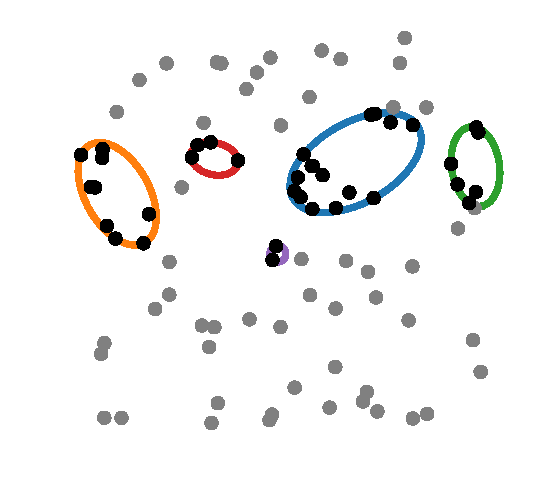
\includegraphics[scale=.9]{figures/MCER_AB108}
	\caption{}
	\label{fig:AB108}
\end{subfigure}
\begin{subfigure}{.5\textwidth}
	\centering
	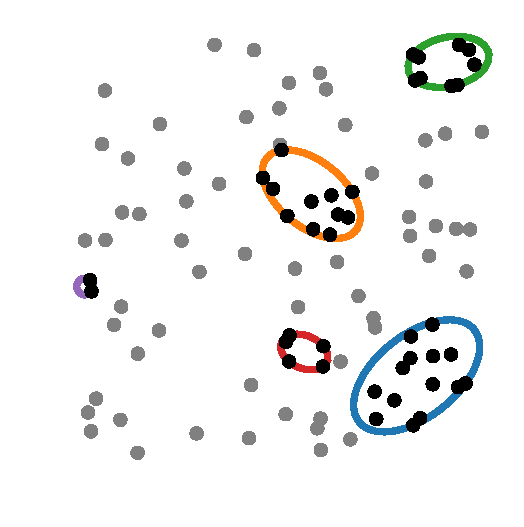
\includegraphics[scale=.9]{figures/MCER_AB120}
	\caption{}
	\label{fig:AB120}
\end{subfigure}
	\caption{An optimal solution of MCER-$k$ for the instance AB108 (a), and for the instance AB120 (b).}
	\label{fig:AB108-AB120}
\end{figure}

\subsection{New instances}

After examining the results obtained for the formerly known instances, we decided to construct new ones to analyze the algorithms proposed by our work more thoroughly. {\color{Red}We were able to run experiments with up to $700$ demand points; however, it is clear that the number of ellipses is the critical parameter of both algorithms, as even for small demand sets, we could not go over $7$ ellipses.}

Besides increasing the size of the demand set and the number of ellipses, we also designed instances with non-unitary weights, which is something none of the previous instances had. 
Moreover, for some instances, we used a different probability distribution, other than the uniform one, to generate the points.
We set a time limit of two hours of CPU time for solving each instance, meaning that if an algorithm did not stop in two hours, we report that it was not able to determine an optimal solution. 
In total, we designed 47 new instances, which will be referred to as TA01, \dots, TA47, and made all of them available at \url{https://sites.icmc.usp.br/andretta/tedeschi-2020/}.

The first set of instances, TA01-TA07, were constructed sampling each demand point from a bivariate normal distribution $\mathcal{N}([0, 0]^T, \mathbb{I})$, with $\mathbb{I} \in \R^{2\times 2}$ being the identity matrix; and setting each point's weight as its squared distance to the origin. This is expected to produce a demand set with most points located near the origin, with the most valuable ones located far away from it.
We generated a set of $n=100$ points, with $m=7$ ellipses, making the $j$-th ellipse have shape parameters randomly taken from a uniform distribution in $[0.5, 1.5]$, and cost $c_j=10\times a_j \times b_j$. From that, we created seven instances for MCE-$k$ and MCER-$k$ taking $k \in \{1, \dots, m\}$. The results for MCE-$k$ are presented in \autoref{tab:mce-results-ta1} and the results for MCER-$k$ are displayed in \autoref{tab:mcer-results-ta1}.
The optimal solutions for the instance TA04 for MCE-$k$ and MCER-$k$ are displayed in \autoref{fig:TA04}. There it is possible to see that because of the normal distribution, most of the points are located close to each other, near the origin, making every ellipse's CLS end up being bigger compared to the previously introduced instances with the same number of demand points. 
This, and the increase in the number of ellipses, made the algorithms for MCER-$k$ and MCE-$k$ time out for some instances. The algorithm for MCER-$k$ did not return an optimal solution within two hours for the instances TA05-TA07, while the algorithm for MCE-$k$ did not finish in time only for the instance TA07. 

For the second set of instances, TA08-TA22, we generated the demand set following the same process as for instances TA01-TA07.
We kept the number of facilities at $3$ and created five demand sets with $n\in\{200, 250, 300, 350, 400\}$. In total, we had $15$ instances with $k\in\{1, \dots, m\}$. The results for MCE-$k$ are displayed in \autoref{tab:mce-results-ta2} and the results for MCER-$k$ are presented in \autoref{tab:mcer-results-ta2}.
Our implementation of the algorithm for MCER-$k$ was not able to obtain a solution for the last instance TA22. Apart from instance TA13 for MCER-$k$, and instance TA22 for both algorithms, most of the CPU time was spent in constructing the CLSs.
The graphical representation of solutions for the instance TA21 for MCE-$k$ and MCER-$k$ are shown in \autoref{fig:TA21}.

The third set of instances, TA23-TA42, was constructed generating each demand point following a uniform distribution in $[0, 10]^2$, with each point having unitary weight; and the ellipses by the same process used for instances TA01-TA23. We created instances with $m=5$, $n\in \{400, 500, 600, 700\}$, and $k\in\{1, \dots, m\}$, with a total of $20$ instances. The results for MCE-$k$ can be seen in \autoref{tab:mce-results-ta3} and the results for MCER-$k$ are presented in \autoref{tab:mcer-results-ta3}. Optimal solutions were obtained for every one of the instances in this set. It is possible to see that, compared with the first two sets of instances, TA01-TA42, the CLS sizes are smaller, mostly because of the size of the ellipses and the uniform distribution used to generate the points. The optimal solution returned by MCER-$k$'s algorithm for the instance TA37 with $n=500$ and $k=5$ is shown in \autoref{fig:TA37}.

The last set of instances, TA43-TA47, were constructed using two bivariate normal distributions with distinct means $\mathcal{N}(\mu^{(1)}, \mathbb{I})$ and $\mathcal{N}(\mu^{(2)}, \mathbb{I})$, $\mu^{(1)}, \mu^{(2)} \in \R^2$. Half of the points were generated following $\mathcal{N}(\mu^{(1)}, \mathbb{I})$, and the other half $\mathcal{N}(\mu^{(2)}, \mathbb{I})$; the weight of every point was set as its squared distance to the mean of the distribution from which it was generated.
The ellipses were also divided into two halves, taking their shape parameters from uniform distributions in the intervals $[0.5, 1.5]$, and $[3, 4]$; setting the $j$-th ellipse's weight as $c_j=a_j \times b_j$.
The purpose of this last set of instances was to create an example where the chosen ellipses in the solution of an instance of MCER-$k$ is not a subset of the chosen ellipses in an optimal solution of that same instance for MCER-$(k+1)$. We created seven instances with $n=80$, $m=6$ and $k\in\{1, \dots, m\}$. We defined the values of $\mu^{(1)}$ and $\mu^{(2)}$ as $(-3, -3)$ and $(-3, -3)$ respectively to create such a counter-example. The results are shown in \autoref{tab:mce-results-ta4} for MCE-$k$ and in \autoref{tab:mcer-results-ta4} for MCER-$k$.
In \autoref{fig:TA44-45}, we show the solutions for the instances TA44-TA45 with $k=2$, where two of the bigger-sized ellipses are used, and $k=3$, where one of the bigger-sized ellipses is replaced by two small ones.

\begin{figure}
\begin{subfigure}{.5\textwidth}
	\centering
	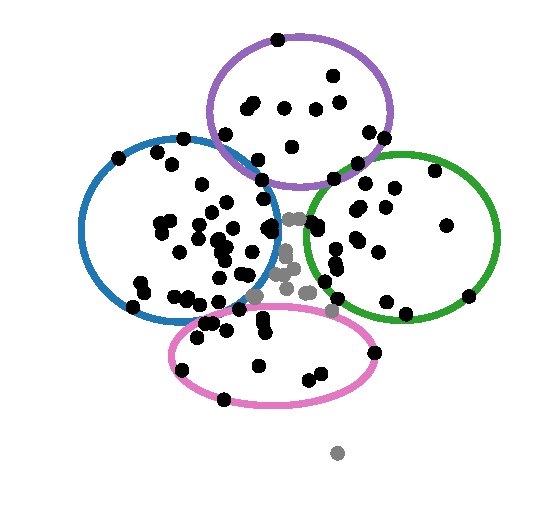
\includegraphics[scale=.9]{figures/MCE_TA04}
	\caption{}
	\label{fig:MCE_TA04}
\end{subfigure}
\begin{subfigure}{.5\textwidth}
	\centering
	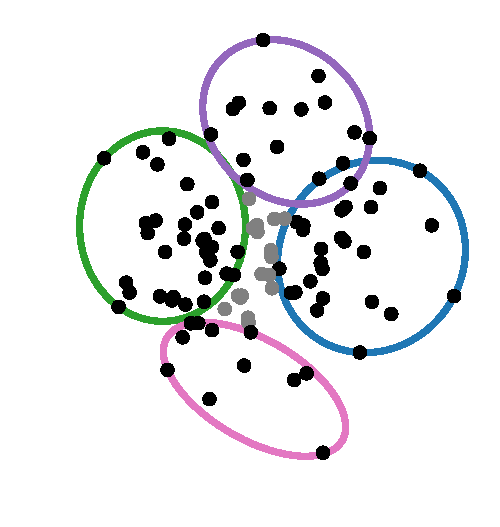
\includegraphics[scale=.9]{figures/MCER_TA04}
	\caption{}
	\label{fig:MCER_TA04}
\end{subfigure}
	\caption{Two optimal solutions for the instance TA04: (a) for MCE-$k$, and (b) for MCER-$k$.}
	\label{fig:TA04}
\end{figure}


\begin{figure}
	\begin{subfigure}{.5\textwidth}
		\centering
		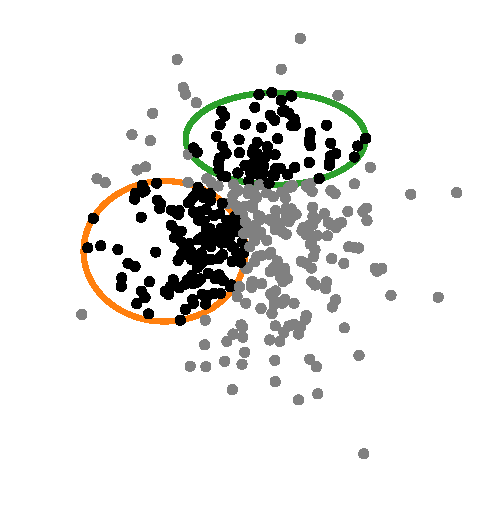
\includegraphics[scale=.9]{figures/MCE_TA21}
		\caption{}
		\label{fig:MCE_TA21}
	\end{subfigure}
	\begin{subfigure}{.5\textwidth}
		\centering
		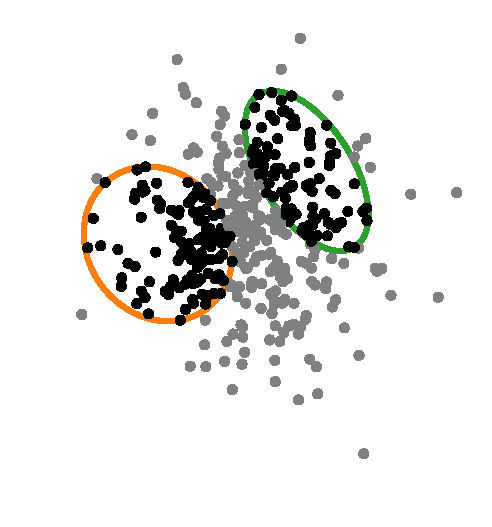
\includegraphics[scale=.9]{figures/MCER_TA21}
		\caption{}
		\label{fig:MCER_TA21}
	\end{subfigure}
	\caption{Two optimal solutions for the instance TA21 with $400$ points: (a) for MCE-$k$, and (b) for MCER-$k$.}
	\label{fig:TA21}
\end{figure}

\begin{figure}
	\begin{subfigure}{.5\textwidth}
		\centering
		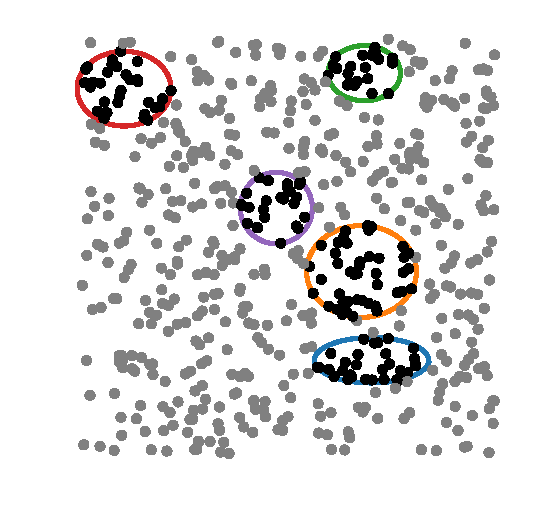
\includegraphics[scale=.9]{figures/MCE_TA37}
		\caption{}
		\label{fig:MCE_TA37}
	\end{subfigure}
	\begin{subfigure}{.5\textwidth}
		\centering
		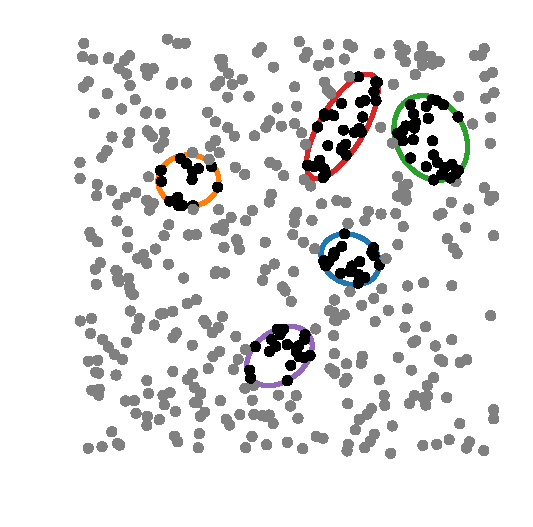
\includegraphics[scale=.9]{figures/MCER_TA37}
		\caption{}
		\label{fig:MCER_TA37}
	\end{subfigure}
	\caption{Two optimal solutions for the instance TA37: (a) for MCE-$k$, and (b) for MCER-$k$.}
	\label{fig:TA37}
\end{figure}

\begin{figure}
	\begin{subfigure}{.5\textwidth}
		\centering
		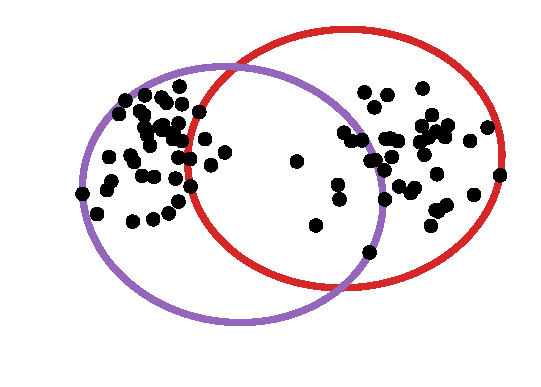
\includegraphics[scale=.9]{figures/MCER_TA44}
		\caption{}
		\label{fig:MCER_TA44}
	\end{subfigure}
	\begin{subfigure}{.5\textwidth}
		\centering
		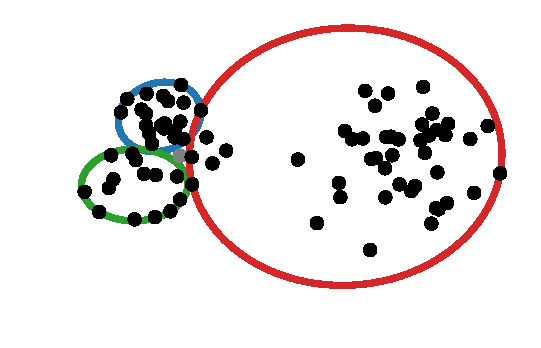
\includegraphics[scale=.9]{figures/MCER_TA45}
		\caption{}
		\label{fig:MCER_TA45}
	\end{subfigure}
	\caption{Two optimal solutions for the instance TA44: (a) for MCE-$k$, and (b) for MCER-$k$.}
	\label{fig:TA44-45}
\end{figure}




%%%% TABLE CM

\begin{table}
	\begin{center}
		\resizebox{\textwidth}{!}{%
			
			\begin{tabular}{|cccc|cr|crrrr|}
				\hline
				\multicolumn{4}{|c|}{Instance} & \multicolumn{2}{c|}{Optimal Solution} & \multicolumn{5}{c|}{Performance metrics}\\
				\hline
				
				%%% Second line of header
				
				\multirow{2}{*}{Name} & 
				\multirow{2}{*}{$n$} & 
				\multirow{2}{*}{$m$} & 
				\multirow{2}{*}{$k$} & 
				Selected & 
				\multirow{2}{*}{Income} & 
				CLS size&
				\multicolumn{2}{c}{Backtracking Tree} & 
				\multicolumn{2}{c|}{\centering CPU Time (s)}\\
				& & & & \centering Ellipses & & $|S_k|$ & \# nodes & \# sol. leaves & CLS-MCE & Total\\
				\hline
				CM1&\multirow{3}{*}{\num{25}}&\multirow{3}{*}{\num{3}}&\num{1}&\num{1}\num{2},\num{3},&\num{3.0}&\num{19}&\num{58}&\num{18}&\num{0.00}&\num{0.00}
\\CM2& & &\num{2}&\num{1},\num{2}\num{3},&\num{3.0}&\num{21}&\num{58}&\num{18}&\num{0.00}&\num{0.00}
\\CM3& & &\num{3}&\num{1},\num{2},\num{3}&\num{3.0}&\num{19}&\num{58}&\num{18}&\num{0.00}&\num{0.00}
\\\hline
CM4&\multirow{3}{*}{\num{50}}&\multirow{3}{*}{\num{3}}&\num{1}&\num{1}\num{2},\num{3},&\num{10.0}&\num{43}&\num{141}&\num{50}&\num{0.00}&\num{0.00}
\\CM5& & &\num{2}&\num{1},\num{2}\num{3},&\num{10.0}&\num{47}&\num{141}&\num{50}&\num{0.00}&\num{0.00}
\\CM6& & &\num{3}&\num{1},\num{2},\num{3}&\num{10.0}&\num{50}&\num{141}&\num{50}&\num{0.00}&\num{0.00}
\\\hline
CM7&\multirow{3}{*}{\num{100}}&\multirow{3}{*}{\num{3}}&\num{1}&\num{1}\num{2},\num{3},&\num{25.0}&\num{101}&\num{924}&\num{687}&\num{0.02}&\num{0.02}
\\CM8& & &\num{2}&\num{1},\num{2}\num{3},&\num{25.0}&\num{135}&\num{924}&\num{687}&\num{0.02}&\num{0.02}
\\CM9& & &\num{3}&\num{1},\num{2},\num{3}&\num{25.0}&\num{174}&\num{924}&\num{687}&\num{0.02}&\num{0.02}
\\
				\hline
				
			\end{tabular}
		}
		\caption{Numerical results of MCE-$k$ for instances CM7-CM9.}
		\label{tab:mce-results-cm}
	\end{center}
\end{table}
%%% TABLE AB
\begin{table}
	\begin{center}
		\resizebox{0.85\textwidth}{!}{%
			
			\begin{tabular}{|cccc|cr|crrrr|}
				\hline
				\multicolumn{4}{|c|}{Instance} & \multicolumn{2}{c|}{Optimal Solution} & \multicolumn{5}{c|}{Performance metrics}\\
				\hline
				
				%%% Second line of header
				\multirow{2}{*}{Name} & 
				\multirow{2}{*}{$n$} & 
				\multirow{2}{*}{$m$} & 
				\multirow{2}{*}{$k$} & 
				Selected & 
				\multirow{2}{*}{Income} & 
				CLS size&
				\multicolumn{2}{c}{Backtracking Tree} & 
				\multicolumn{2}{c|}{\centering CPU Time (s)}\\
				& & & & \centering Ellipses & & $|S_k|$ & \# nodes & \# sol. leaves & CLS-MCE & Total\\
				\hline
				AB097&\multirow{3}{*}{\num{90}}&\multirow{3}{*}{\num{3}}&\num{1}&\num{1}&\num{5.5}&\num{77}&\num{439}&\num{216}&\num{0.02}&\num{0.02}
\\AB098& & &\num{2}&\num{1},\num{2}&\num{9.9}&\num{63}&\num{561}&\num{203}&\num{0.02}&\num{0.02}
\\AB099& & &\num{3}&\num{1},\num{2},\num{3}&\num{11.8}&\num{76}&\num{205}&\num{67}&\num{0.02}&\num{0.02}
\\\hline
AB100&\multirow{4}{*}{\num{90}}&\multirow{4}{*}{\num{4}}&\num{1}&\num{1}&\num{6.2}&\num{87}&\num{757}&\num{292}&\num{0.02}&\num{0.02}
\\AB101& & &\num{2}&\num{1},\num{2}&\num{10.7}&\num{68}&\num{1424}&\num{395}&\num{0.02}&\num{0.02}
\\AB102& & &\num{3}&\num{1},\num{2},\num{3}&\num{14.1}&\num{58}&\num{1030}&\num{260}&\num{0.02}&\num{0.02}
\\AB103& & &\num{4}&\num{1},\num{2},\num{3},\num{4}&\num{17.0}&\num{79}&\num{267}&\num{65}&\num{0.02}&\num{0.02}
\\\hline
AB104&\multirow{5}{*}{\num{90}}&\multirow{5}{*}{\num{5}}&\num{1}&\num{2}&\num{8.2}&\num{130}&\num{770}&\num{287}&\num{0.04}&\num{0.04}
\\AB105& & &\num{2}&\num{2},\num{3}&\num{12.7}&\num{96}&\num{1522}&\num{365}&\num{0.04}&\num{0.04}
\\AB106& & &\num{3}&\num{1},\num{2},\num{3}&\num{16.2}&\num{61}&\num{9612}&\num{352}&\num{0.04}&\num{0.04}
\\AB107& & &\num{4}&\num{1},\num{2},\num{3},\num{4}&\num{19.6}&\num{58}&\num{26173}&\num{206}&\num{0.04}&\num{0.05}
\\AB108& & &\num{5}&\num{1},\num{2},\num{3},\num{4},\num{5}&\num{21.5}&\num{72}&\num{16033}&\num{211}&\num{0.04}&\num{0.05}
\\\hline
AB109&\multirow{3}{*}{\num{100}}&\multirow{3}{*}{\num{3}}&\num{1}&\num{1}&\num{5.5}&\num{90}&\num{511}&\num{249}&\num{0.02}&\num{0.02}
\\AB110& & &\num{2}&\num{1},\num{2}&\num{10.9}&\num{76}&\num{653}&\num{230}&\num{0.02}&\num{0.02}
\\AB111& & &\num{3}&\num{1},\num{2},\num{3}&\num{13.8}&\num{83}&\num{238}&\num{74}&\num{0.02}&\num{0.02}
\\\hline
AB112&\multirow{4}{*}{\num{100}}&\multirow{4}{*}{\num{4}}&\num{1}&\num{1}&\num{7.2}&\num{119}&\num{928}&\num{339}&\num{0.03}&\num{0.03}
\\AB113& & &\num{2}&\num{1},\num{2}&\num{12.7}&\num{80}&\num{1705}&\num{411}&\num{0.03}&\num{0.03}
\\AB114& & &\num{3}&\num{1},\num{2},\num{3}&\num{17.1}&\num{62}&\num{1217}&\num{258}&\num{0.03}&\num{0.03}
\\AB115& & &\num{4}&\num{1},\num{2},\num{3},\num{4}&\num{20.0}&\num{78}&\num{313}&\num{63}&\num{0.03}&\num{0.03}
\\\hline
AB116&\multirow{5}{*}{\num{100}}&\multirow{5}{*}{\num{5}}&\num{1}&\num{1}&\num{8.5}&\num{142}&\num{1185}&\num{376}&\num{0.05}&\num{0.05}
\\AB117& & &\num{2}&\num{1},\num{3}&\num{16.0}&\num{119}&\num{1445}&\num{369}&\num{0.05}&\num{0.05}
\\AB118& & &\num{3}&\num{1},\num{2},\num{3}&\num{22.2}&\num{76}&\num{1815}&\num{338}&\num{0.05}&\num{0.05}
\\AB119& & &\num{4}&\num{1},\num{2},\num{3},\num{4}&\num{25.6}&\num{74}&\num{1796}&\num{249}&\num{0.05}&\num{0.05}
\\AB120& & &\num{5}&\num{1},\num{2},\num{3},\num{4},\num{5}&\num{27.5}&\num{84}&\num{723}&\num{118}&\num{0.05}&\num{0.05}
\\
				\hline
				
			\end{tabular}
		}
		\caption{Numerical results of MCE-$k$ for instances AB097-AB120.}
		\label{tab:mce-results-ab}
	\end{center}
\end{table}


\begin{table}
	\begin{center}
		\resizebox{\textwidth}{!}{%
			
			\begin{tabular}{|cccc|cr|ccrrrr|}
				\hline
				\multicolumn{4}{|c|}{Instance} & \multicolumn{2}{c|}{Optimal Solution} & \multicolumn{6}{c|}{Performance metrics}\\
				\hline
				
				%%% Second line of header
				
				\multirow{2}{*}{Name} & 
				\multirow{2}{*}{$n$} & 
				\multirow{2}{*}{$m$} & 
				\multirow{2}{*}{$k$} & 
				Selected & 
				\multirow{2}{*}{Income} & 
				CLS size&
				\# E3P&
				\multicolumn{2}{c}{Backtracking Tree} & 
				\multicolumn{2}{c|}{\centering CPU Time (s)}\\
				& & & & \centering Ellipses & & $|S_k|$ & subproblems & \# nodes & \# sol leaves & CLS-MCER & Total\\
				
				%%%
				%%%
				
				\hline
				CM1&\multirow{3}{*}{\num{25}}&\multirow{3}{*}{\num{3}}&\num{1}&\num{1}&\num{2.0}&\num{27}&\num{480}&\num{82}&\num{27}&\num{0.09}&\num{0.09}
\\CM2& & &\num{2}&\num{1},\num{2}&\num{4.8}&\num{24}&\num{480}&\num{124}&\num{48}&\num{0.09}&\num{0.09}
\\CM3& & &\num{3}&\num{1},\num{2},\num{3}&\num{5.0}&\num{37}&\num{480}&\num{224}&\num{148}&\num{0.09}&\num{0.09}
\\\hline
CM4&\multirow{3}{*}{\num{50}}&\multirow{3}{*}{\num{3}}&\num{1}&\num{1}&\num{4.0}&\num{70}&\num{3427}&\num{211}&\num{70}&\num{0.62}&\num{0.62}
\\CM5& & &\num{2}&\num{1},\num{2}&\num{9.8}&\num{89}&\num{3427}&\num{427}&\num{178}&\num{0.62}&\num{0.62}
\\CM6& & &\num{3}&\num{1},\num{2},\num{3}&\num{13.0}&\num{111}&\num{3427}&\num{582}&\num{333}&\num{0.63}&\num{0.63}
\\\hline
CM7&\multirow{3}{*}{\num{100}}&\multirow{3}{*}{\num{3}}&\num{1}&\num{1}&\num{8.0}&\num{201}&\num{32242}&\num{604}&\num{201}&\num{7.85}&\num{7.85}
\\CM8& & &\num{2}&\num{1},\num{2}&\num{17.8}&\num{369}&\num{32242}&\num{1678}&\num{738}&\num{7.88}&\num{7.88}
\\CM9& & &\num{3}&\num{1},\num{2},\num{3}&\num{28.0}&\num{701}&\num{32242}&\num{4438}&\num{3498}&\num{7.83}&\num{7.86}
\\
				\hline
				
			\end{tabular}
		}
		\caption{Numerical results of MCER-$k$ for instances CM7-CM9.}
		\label{tab:mcer-results-cm}
	\end{center}
\end{table}

%%% FIM TABLE CM

\begin{table}
	\begin{center}
		\resizebox{\textwidth}{!}{%
			
			\begin{tabular}{|cccc|cr|ccrrrr|}
				\hline
				\multicolumn{4}{|c|}{Instance} & \multicolumn{2}{c|}{Optimal Solution} & \multicolumn{6}{c|}{Performance metrics}\\
				\hline
				
				%%% Second line of header
				
				\multirow{2}{*}{Name} & 
				\multirow{2}{*}{$n$} & 
				\multirow{2}{*}{$m$} & 
				\multirow{2}{*}{$k$} & 
				Selected & 
				\multirow{2}{*}{Income} & 
				CLS size&
				\# E3P&
				\multicolumn{2}{c}{Backtracking Tree} & 
				\multicolumn{2}{c|}{\centering CPU Time (s)}\\
				& & & & \centering Ellipses & & $|S_k|$ & subproblems & \# nodes & \# sol leaves & CLS-MCER & Total\\
				
				%%%%
				%%%%
				
				
				\hline
				AB097&\multirow{3}{*}{\num{90}}&\multirow{3}{*}{\num{3}}&\num{1}&\num{1}&\num{5.5}&\num{160}&\multirow{3}{*}{\num{1157}}&\num{728}&\num{319}&\num{0.29}&\num{0.29}
\\AB098& & &\num{2}&\num{1},\num{2}&\num{9.9}&\num{83}& &\num{866}&\num{221}&\num{0.28}&\num{0.28}
\\AB099& & &\num{3}&\num{1},\num{2},\num{3}&\num{11.8}&\num{76}& &\num{306}&\num{67}&\num{0.29}&\num{0.29}
\\\hline
AB100&\multirow{4}{*}{\num{90}}&\multirow{4}{*}{\num{4}}&\num{1}&\num{1}&\num{7.2}&\num{207}&\multirow{4}{*}{\num{3019}}&\num{1465}&\num{494}&\num{0.72}&\num{0.73}
\\AB101& & &\num{2}&\num{1},\num{2}&\num{12.7}&\num{132}& &\num{2593}&\num{481}&\num{0.73}&\num{0.73}
\\AB102& & &\num{3}&\num{1},\num{2},\num{3}&\num{16.1}&\num{76}& &\num{1800}&\num{261}&\num{0.74}&\num{0.74}
\\AB103& & &\num{4}&\num{1},\num{2},\num{3},\num{4}&\num{19.0}&\num{79}& &\num{455}&\num{61}&\num{0.72}&\num{0.72}
\\\hline
AB104&\multirow{5}{*}{\num{90}}&\multirow{5}{*}{\num{5}}&\num{1}&\num{1}&\num{10.5}&\num{452}&\multirow{5}{*}{\num{10488}}&\num{2820}&\num{703}&\num{2.46}&\num{2.46}
\\AB105& & &\num{2}&\num{1},\num{2}&\num{16.7}&\num{249}& &\num{5862}&\num{704}&\num{2.48}&\num{2.48}
\\AB106& & &\num{3}&\num{1},\num{2},\num{3}&\num{21.2}&\num{115}& &\num{13041}&\num{434}&\num{2.48}&\num{2.49}
\\AB107& & &\num{4}&\num{1},\num{2},\num{3},\num{4}&\num{24.6}&\num{64}& &\num{72194}&\num{501}&\num{2.56}&\num{2.60}
\\AB108& & &\num{5}&\num{1},\num{2},\num{3},\num{4},\num{5}&\num{26.5}&\num{72}& &\num{105181}&\num{312}&\num{2.46}&\num{2.51}
\\\hline
AB109&\multirow{3}{*}{\num{100}}&\multirow{3}{*}{\num{3}}&\num{1}&\num{1}&\num{7.5}&\num{181}&\multirow{3}{*}{\num{1614}}&\num{836}&\num{366}&\num{0.39}&\num{0.39}
\\AB110& & &\num{2}&\num{1},\num{2}&\num{12.9}&\num{102}& &\num{1002}&\num{255}&\num{0.41}&\num{0.41}
\\AB111& & &\num{3}&\num{1},\num{2},\num{3}&\num{15.8}&\num{83}& &\num{354}&\num{74}&\num{0.40}&\num{0.40}
\\\hline
AB112&\multirow{4}{*}{\num{100}}&\multirow{4}{*}{\num{4}}&\num{1}&\num{1}&\num{8.2}&\num{337}&\multirow{4}{*}{\num{5613}}&\num{2091}&\num{660}&\num{1.33}&\num{1.33}
\\AB113& & &\num{2}&\num{1},\num{2}&\num{14.7}&\num{165}& &\num{3604}&\num{527}&\num{1.35}&\num{1.35}
\\AB114& & &\num{3}&\num{1},\num{2},\num{3}&\num{19.1}&\num{80}& &\num{2487}&\num{270}&\num{1.32}&\num{1.32}
\\AB115& & &\num{4}&\num{1},\num{2},\num{3},\num{4}&\num{22.0}&\num{78}& &\num{629}&\num{62}&\num{1.33}&\num{1.33}
\\\hline
AB116&\multirow{5}{*}{\num{100}}&\multirow{5}{*}{\num{5}}&\num{1}&\num{1}&\num{9.5}&\num{649}&\multirow{5}{*}{\num{14029}}&\num{5571}&\num{1387}&\num{3.31}&\num{3.31}
\\AB117& & &\num{2}&\num{1},\num{2}&\num{17.7}&\num{368}& &\num{6671}&\num{1031}&\num{3.30}&\num{3.30}
\\AB118& & &\num{3}&\num{1},\num{2},\num{3}&\num{25.2}&\num{183}& &\num{7344}&\num{609}&\num{3.32}&\num{3.32}
\\AB119& & &\num{4}&\num{1},\num{2},\num{3},\num{4}&\num{29.6}&\num{103}& &\num{6474}&\num{320}&\num{3.32}&\num{3.33}
\\AB120& & &\num{5}&\num{1},\num{2},\num{3},\num{4},\num{5}&\num{31.5}&\num{84}& &\num{1579}&\num{119}&\num{3.30}&\num{3.30}
\\
				\hline
				
			\end{tabular}
		}
		\caption{Numerical results of MCER-$k$ for instances AB097-AB120.}
		\label{tab:mcer-results-ab}
	\end{center}
\end{table}

%%% FIM TABLE AB
%%%% NEW INSTANCES





\begin{table}
	\begin{center}
		\resizebox{\textwidth}{!}{%
			
			\begin{tabular}{|cccc|cr|crrrr|}
				\hline
				\multicolumn{4}{|c|}{Instance} & \multicolumn{2}{c|}{Optimal Solution} & \multicolumn{5}{c|}{Performance metrics}\\
				\hline
				
				%%% Second line of header
				
				\multirow{2}{*}{Name} & 
				\multirow{2}{*}{$n$} & 
				\multirow{2}{*}{$m$} & 
				\multirow{2}{*}{$k$} & 
				Selected & 
				\multirow{2}{*}{Income} & 
				CLS size&
				\multicolumn{2}{c}{Backtracking Tree} & 
				\multicolumn{2}{c|}{\centering CPU Time (s)}\\
				& & & & \centering Ellipses & & $|S_k|$ & \# nodes & \# sol leaves & CLS-MCER & Total\\
				
				%%%%
				%%%%
				
				
				\hline
				TA001&\multirow{8}{*}{\num{100}}&\multirow{8}{*}{\num{8}}&\num{1}&\num{1}&\num{27.5}&\num{205}&\num{1641}&\num{205}&\num{0.22}&\num{0.22}
\\TA002& & &\num{2}&\num{1},\num{2}&\num{56.3}&\num{188}&\num{1522}&\num{188}&\num{0.22}&\num{0.22}
\\TA003& & &\num{3}&\num{1},\num{2},\num{3}&\num{83.6}&\num{212}&\num{2938}&\num{424}&\num{0.22}&\num{0.23}
\\TA004& & &\num{4}&\num{1},\num{2},\num{3},\num{4}&\num{100.6}&\num{209}&\num{10726}&\num{1389}&\num{0.22}&\num{0.28}
\\TA005& & &\num{5}&\num{1},\num{2},\num{3},\num{4},\num{5}&\num{117.5}&\num{184}&\num{10172}&\num{2191}&\num{0.22}&\num{0.27}
\\TA006& & &\num{6}&\num{1},\num{2},\num{3},\num{4},\num{5},\num{6}&\num{130.6}&\num{204}&\num{28575}&\num{5293}&\num{0.21}&\num{0.72}
\\TA007& & &\num{7}&\num{1},\num{2},\num{3},\num{4},\num{5},\num{6},\num{7}&\num{129.7}&\num{186}&\num{10498}&\num{3399}&\num{0.22}&\num{0.34}
\\TA008& & &\num{8}&\num{1},\num{2},\num{3},\num{4},\num{5},\num{6},\num{7},\num{8}&\num{128.9}&\num{200}&\num{10816}&\num{4280}&\num{0.22}&\num{0.46}
\\
				\hline
				
			\end{tabular}
		}
		\caption{Numerical results of MCE-$k$ for instances TA001-TA007.}
		\label{tab:mce-results-ta1}
	\end{center}
\end{table}

\begin{table}
	\begin{center}
		\resizebox{\textwidth}{!}{%
			
			\begin{tabular}{|cccc|cr|crrrr|}
				\hline
				\multicolumn{4}{|c|}{Instance} & \multicolumn{2}{c|}{Optimal Solution} & \multicolumn{5}{c|}{Performance metrics}\\
				\hline
				
				%%% Second line of header
				
				\multirow{2}{*}{Name} & 
				\multirow{2}{*}{$n$} & 
				\multirow{2}{*}{$m$} & 
				\multirow{2}{*}{$k$} & 
				Selected & 
				\multirow{2}{*}{Income} & 
				CLS size&
				\multicolumn{2}{c}{Backtracking Tree} & 
				\multicolumn{2}{c|}{\centering CPU Time (s)}\\
				& & & & \centering Ellipses & & $|S_k|$ & \# nodes & \# sol leaves & CLS-MCER & Total\\
				
				%%%%
				%%%%
				
				%%%%
				%%%%
				
				
				\hline
				TA008&\multirow{3}{*}{\num{200}}&\multirow{3}{*}{\num{3}}&\num{1}&\num{2}&\num{82.1}&\num{836}&\num{2577}&\num{1760}&\num{1.19}&\num{1.19}
\\TA009& & &\num{2}&\num{1},\num{2}&\num{157.2}&\num{811}&\num{9993}&\num{4238}&\num{1.19}&\num{1.21}
\\TA010& & &\num{3}&\num{1},\num{2},\num{3}&\num{192.6}&\num{949}&\num{38939}&\num{7294}&\num{1.19}&\num{1.31}
\\\hline
TA011&\multirow{3}{*}{\num{250}}&\multirow{3}{*}{\num{3}}&\num{1}&\num{2}&\num{103.4}&\num{1349}&\num{3845}&\num{2610}&\num{2.11}&\num{2.11}
\\TA012& & &\num{2}&\num{2},\num{3}&\num{196.5}&\num{1229}&\num{3995}&\num{2762}&\num{1.95}&\num{1.96}
\\TA013& & &\num{3}&\num{1},\num{2},\num{3}&\num{249.0}&\num{1381}&\num{23598}&\num{12416}&\num{1.96}&\num{2.09}
\\\hline
TA014&\multirow{3}{*}{\num{300}}&\multirow{3}{*}{\num{3}}&\num{1}&\num{1}&\num{112.1}&\num{2128}&\num{8493}&\num{4231}&\num{2.95}&\num{2.96}
\\TA015& & &\num{2}&\num{1},\num{3}&\num{207.7}&\num{2152}&\num{10602}&\num{4190}&\num{3.00}&\num{3.01}
\\TA016& & &\num{3}&\num{1},\num{2},\num{3}&\num{299.4}&\num{2103}&\num{12726}&\num{4181}&\num{2.97}&\num{2.99}
\\\hline
TA017&\multirow{3}{*}{\num{350}}&\multirow{3}{*}{\num{3}}&\num{1}&\num{2}&\num{224.4}&\num{2561}&\num{6487}&\num{4550}&\num{9.54}&\num{9.55}
\\TA018& & &\num{2}&\num{1},\num{2}&\num{379.7}&\num{1931}&\num{14030}&\num{7603}&\num{10.47}&\num{10.54}
\\TA019& & &\num{3}&\num{1},\num{2},\num{3}&\num{460.1}&\num{2619}&\num{197645}&\num{17431}&\num{10.24}&\num{12.01}
\\

				\hline
				%TA014&\multirow{3}{*}{\num{300}}&\multirow{3}{*}{\num{3}}&\num{1}&\num{1}&\num{112.1}&\num{6693}&\multirow{3}{*}{\num{1755415}}&\num{42702}&\num{29310}&\num{383.00}&\num{383.05}
\\TA015& & &\num{2}&\num{1},\num{3}&\num{214.2}&\num{22954}& &\num{81519}&\num{45175}&\num{410.92}&\num{411.05}
\\TA016& & &\num{3}&\num{1},\num{2},\num{3}&\num{311.2}&\num{22617}& &\num{257865}&\num{22558}&\num{401.90}&\num{402.44}
\\

				%\hline
				
			\end{tabular}
		}
		\caption{Numerical results of MCE-$k$ for instances TA008-TA022.}
		
		\label{tab:mce-results-ta2}
	\end{center}
\end{table}

\begin{table}
	\begin{center}
		\resizebox{\textwidth}{!}{%
			
			\begin{tabular}{|cccc|cr|crrrr|}
				\hline
				\multicolumn{4}{|c|}{Instance} & \multicolumn{2}{c|}{Optimal Solution} & \multicolumn{5}{c|}{Performance metrics}\\
				\hline
				
				%%% Second line of header
				
				\multirow{2}{*}{Name} & 
				\multirow{2}{*}{$n$} & 
				\multirow{2}{*}{$m$} & 
				\multirow{2}{*}{$k$} & 
				Selected & 
				\multirow{2}{*}{Income} & 
				CLS size&
				\multicolumn{2}{c}{Backtracking Tree} & 
				\multicolumn{2}{c|}{\centering CPU Time (s)}\\
				& & & & \centering Ellipses & & $|S_k|$ & \# nodes & \# sol leaves & CLS-MCER & Total\\
				
				%%%%
				%%%%
				
				%%%%
				%%%%
				
				
				\hline
				TA23&\multirow{5}{*}{\num{400}}&\multirow{5}{*}{\num{5}}&\num{1}&\num{5}&\num{14.5}&\num{830}&\num{1165}&\num{1150}&\num{0.96}&\num{0.96}
\\TA24& & &\num{2}&\num{3},\num{5}&\num{27.4}&\num{627}&\num{2930}&\num{1150}&\num{0.95}&\num{0.95}
\\TA25& & &\num{3}&\num{3},\num{4},\num{5}&\num{36.8}&\num{880}&\num{26520}&\num{3450}&\num{0.95}&\num{0.97}
\\TA26& & &\num{4}&\num{1},\num{3},\num{4},\num{5}&\num{46.2}&\num{660}&\num{587336}&\num{9200}&\num{0.95}&\num{1.48}
\\TA27& & &\num{5}&\num{1},\num{2},\num{3},\num{4},\num{5}&\num{54.2}&\num{1150}&\num{5715962}&\num{18356}&\num{0.95}&\num{9.91}
\\\hline
TA28&\multirow{5}{*}{\num{500}}&\multirow{5}{*}{\num{5}}&\num{1}&\num{4}&\num{30.9}&\num{1396}&\num{4071}&\num{2028}&\num{2.48}&\num{2.48}
\\TA29& & &\num{2}&\num{4},\num{5}&\num{57.8}&\num{1256}&\num{3983}&\num{1935}&\num{2.52}&\num{2.53}
\\TA30& & &\num{3}&\num{3},\num{4},\num{5}&\num{80.9}&\num{1678}&\num{19478}&\num{9673}&\num{2.53}&\num{2.56}
\\TA31& & &\num{4}&\num{1},\num{3},\num{4},\num{5}&\num{101.3}&\num{2028}&\num{101334}&\num{9674}&\num{2.50}&\num{2.67}
\\TA32& & &\num{5}&\num{1},\num{2},\num{3},\num{4},\num{5}&\num{117.7}&\num{1939}&\num{2040107}&\num{17428}&\num{2.56}&\num{6.11}
\\\hline
TA33&\multirow{5}{*}{\num{600}}&\multirow{5}{*}{\num{5}}&\num{1}&\num{2}&\num{42.5}&\num{1980}&\num{14067}&\num{3513}&\num{4.79}&\num{4.80}
\\TA34& & &\num{2}&\num{2},\num{4}&\num{73.5}&\num{3513}&\num{12372}&\num{2663}&\num{4.70}&\num{4.71}
\\TA35& & &\num{3}&\num{1},\num{2},\num{4}&\num{101.8}&\num{1713}&\num{19671}&\num{5325}&\num{4.80}&\num{4.82}
\\TA36& & &\num{4}&\num{1},\num{2},\num{4},\num{5}&\num{126.0}&\num{2696}&\num{24966}&\num{7960}&\num{4.71}&\num{4.73}
\\TA37& & &\num{5}&\num{1},\num{2},\num{3},\num{4},\num{5}&\num{147.4}&\num{2047}&\num{70594}&\num{7949}&\num{4.74}&\num{4.81}
\\\hline
TA38&\multirow{5}{*}{\num{700}}&\multirow{5}{*}{\num{5}}&\num{1}&\num{5}&\num{63.0}&\num{4635}&\num{5557}&\num{5542}&\num{8.96}&\num{8.97}
\\TA39& & &\num{2}&\num{1},\num{5}&\num{110.5}&\num{3243}&\num{24102}&\num{5542}&\num{9.06}&\num{9.12}
\\TA40& & &\num{3}&\num{1},\num{2},\num{5}&\num{143.6}&\num{2212}&\num{19804}&\num{5542}&\num{9.06}&\num{9.46}
\\TA41& & &\num{4}&\num{1},\num{2},\num{4},\num{5}&\num{169.9}&\num{2536}&\num{341942}&\num{44336}&\num{9.04}&\num{14.92}
\\TA42& & &\num{5}&\num{1},\num{2},\num{3},\num{4},\num{5}&\num{195.3}&\num{5542}&\num{506117}&\num{49878}&\num{9.00}&\num{22.39}
\\

				\hline
				%TA014&\multirow{3}{*}{\num{300}}&\multirow{3}{*}{\num{3}}&\num{1}&\num{1}&\num{112.1}&\num{6693}&\multirow{3}{*}{\num{1755415}}&\num{42702}&\num{29310}&\num{383.00}&\num{383.05}
\\TA015& & &\num{2}&\num{1},\num{3}&\num{214.2}&\num{22954}& &\num{81519}&\num{45175}&\num{410.92}&\num{411.05}
\\TA016& & &\num{3}&\num{1},\num{2},\num{3}&\num{311.2}&\num{22617}& &\num{257865}&\num{22558}&\num{401.90}&\num{402.44}
\\

				%\hline
				
			\end{tabular}
		}
		\caption{Numerical results of MCE-$k$ for instances TA023-TA042.}
		\label{tab:mce-results-ta3}
	\end{center}
\end{table}

\begin{table}
	\begin{center}
		\resizebox{\textwidth}{!}{%
			
			\begin{tabular}{|cccc|cr|crrrr|}
				\hline
				\multicolumn{4}{|c|}{Instance} & \multicolumn{2}{c|}{Optimal Solution} & \multicolumn{5}{c|}{Performance metrics}\\
				\hline
				
				%%% Second line of header
				
				\multirow{2}{*}{Name} & 
				\multirow{2}{*}{$n$} & 
				\multirow{2}{*}{$m$} & 
				\multirow{2}{*}{$k$} & 
				Selected & 
				\multirow{2}{*}{Income} & 
				CLS size&
				\multicolumn{2}{c}{Backtracking Tree} & 
				\multicolumn{2}{c|}{\centering CPU Time (s)}\\
				& & & & \centering Ellipses & & $|S_k|$ & \# nodes & \# sol leaves & CLS-MCER & Total\\

				
				
				\hline
				TA43&\multirow{5}{*}{\num{80}}&\multirow{5}{*}{\num{5}}&\num{1}&\num{5}&\num{87.9}&\num{97}&\num{43}&\num{28}&\num{0.22}&\num{0.22}
\\TA44& & &\num{2}&\num{3},\num{4}&\num{126.9}&\num{89}&\num{314}&\num{95}&\num{0.21}&\num{0.22}
\\TA45& & &\num{3}&\num{1},\num{2},\num{3}&\num{136.8}&\num{39}&\num{33898}&\num{229}&\num{0.21}&\num{0.43}
\\TA46& & &\num{4}&\num{1},\num{2},\num{3},\num{4}&\num{124.8}&\num{42}&\num{1689010}&\num{146}&\num{0.21}&\num{11.71}
\\TA47& & &\num{5}&\num{1},\num{2},\num{3},\num{4},\num{5}&\num{110.3}&\num{28}&\num{12794063}&\num{1}&\num{0.22}&\num{101.23}
\\
				\hline
				%TA014&\multirow{3}{*}{\num{300}}&\multirow{3}{*}{\num{3}}&\num{1}&\num{1}&\num{112.1}&\num{6693}&\multirow{3}{*}{\num{1755415}}&\num{42702}&\num{29310}&\num{383.00}&\num{383.05}
\\TA015& & &\num{2}&\num{1},\num{3}&\num{214.2}&\num{22954}& &\num{81519}&\num{45175}&\num{410.92}&\num{411.05}
\\TA016& & &\num{3}&\num{1},\num{2},\num{3}&\num{311.2}&\num{22617}& &\num{257865}&\num{22558}&\num{401.90}&\num{402.44}
\\

				%\hline
				
			\end{tabular}
		}
		\caption{Numerical results of MCE-$k$ for instances TA043-TA047.}
		
		\label{tab:mce-results-ta4}
	\end{center}
\end{table}


\begin{table}
	\begin{center}
		\resizebox{\textwidth}{!}{%
			
			\begin{tabular}{|cccc|cr|ccrrrr|}
				\hline
				\multicolumn{4}{|c|}{Instance} & \multicolumn{2}{c|}{Optimal Solution} & \multicolumn{6}{c|}{Performance metrics}\\
				\hline
				
				%%% Second line of header
				
				\multirow{2}{*}{Name} & 
				\multirow{2}{*}{$n$} & 
				\multirow{2}{*}{$m$} & 
				\multirow{2}{*}{$k$} & 
				Selected & 
				\multirow{2}{*}{Income} & 
				CLS size&
				\# E3P&
				\multicolumn{2}{c}{Backtracking Tree} & 
				\multicolumn{2}{c|}{\centering CPU Time (s)}\\
				& & & & \centering Ellipses & & $|S_k|$ & subproblems & \# nodes & \# sol leaves & CLS-MCER & Total\\
				
				
				\hline
				TA01&\multirow{7}{*}{\num{100}}&\multirow{7}{*}{\num{7}}&\num{1}&\num{3}&\num{52.4}&\num{470}&\multirow{7}{*}{\num{146116}}&\num{10026}&\num{4830}&\num{43.26}&\num{43.27}
\\TA02& & &\num{2}&\num{1},\num{3}&\num{102.3}&\num{3015}& &\num{30072}&\num{11475}&\num{43.21}&\num{43.23}
\\TA03& & &\num{3}&\num{1},\num{3},\num{5}&\num{135.2}&\num{755}& &\num{1259300}&\num{24958}&\num{43.28}&\num{46.97}
\\TA04& & &\num{4}&\num{1},\num{3},\num{5},\num{7}&\num{157.1}&\num{721}& &\num{57430353}&\num{74709}&\num{43.30}&\num{462.09}
\\TA05& & &5&-&-&1059& &-&-&-&-
\\TA06& & &6&-&-&973& &-&-&-&-
\\TA07& & &7&-&-&3132& &-&-&-&-\\
				\hline
				
			\end{tabular}
		}
		\caption{Numerical results of MCER-$k$ for instances TA001-TA007.}
		\label{tab:mcer-results-ta1}
	\end{center}
\end{table}



\begin{table}
	\begin{center}
		\resizebox{\textwidth}{!}{%
			
			\begin{tabular}{|cccc|cr|ccrrrr|}
				\hline
				\multicolumn{4}{|c|}{Instance} & \multicolumn{2}{c|}{Optimal Solution} & \multicolumn{6}{c|}{Performance metrics}\\
				\hline
				
				%%% Second line of header
				
				\multirow{2}{*}{Name} & 
				\multirow{2}{*}{$n$} & 
				\multirow{2}{*}{$m$} & 
				\multirow{2}{*}{$k$} & 
				Selected & 
				\multirow{2}{*}{Income} & 
				CLS size&
				\# E3P&
				\multicolumn{2}{c}{Backtracking Tree} & 
				\multicolumn{2}{c|}{\centering CPU Time (s)}\\
				& & & & \centering Ellipses & & $|S_k|$ & subproblems & \# nodes & \# sol leaves & CLS-MCER & Total\\
				
				
				\hline
				TA008&\multirow{3}{*}{\num{200}}&\multirow{3}{*}{\num{3}}&\num{1}&\num{1}&\num{85.9}&\num{8589}&\multirow{3}{*}{\num{681627}}&\num{37146}&\num{18514}&\num{129.71}&\num{129.73}
\\TA009& & &\num{2}&\num{1},\num{2}&\num{169.7}&\num{1448}& &\num{53908}&\num{25243}&\num{129.22}&\num{129.27}
\\TA010& & &\num{3}&\num{1},\num{2},\num{3}&\num{202.6}&\num{8477}& &\num{772760}&\num{60542}&\num{128.75}&\num{138.25}
\\\hline
TA011&\multirow{3}{*}{\num{250}}&\multirow{3}{*}{\num{3}}&\num{1}&\num{2}&\num{126.2}&\num{11226}&\multirow{3}{*}{\num{995713}}&\num{59486}&\num{34196}&\num{228.61}&\num{228.68}
\\TA012& & &\num{2}&\num{2},\num{3}&\num{215.0}&\num{25284}& &\num{34200}&\num{8912}&\num{232.41}&\num{233.87}
\\
TA013 & & & \num{3} & \num{1},\num{2},\num{3} & \num{262.8} & \num{8912} & & \num{32908602} & \num{53459} & \num{226.03} & \num{610.32}
\\\hline
TA014&\multirow{3}{*}{\num{300}}&\multirow{3}{*}{\num{3}}&\num{1}&\num{1}&\num{112.1}&\num{6693}&\multirow{3}{*}{\num{1755415}}&\num{42702}&\num{29310}&\num{383.00}&\num{383.05}
\\TA015& & &\num{2}&\num{1},\num{3}&\num{214.2}&\num{22954}& &\num{81519}&\num{45175}&\num{410.92}&\num{411.05}
\\TA016& & &\num{3}&\num{1},\num{2},\num{3}&\num{311.2}&\num{22617}& &\num{257865}&\num{22558}&\num{401.90}&\num{402.44}
\\\hline
TA017&\multirow{3}{*}{\num{350}}&\multirow{3}{*}{\num{3}}&\num{1}&\num{2}&\num{225.9}&\num{63315}&\multirow{3}{*}{\num{2961709}}&\num{54419}&\num{43151}&\num{775.78}&\num{775.85}
\\TA018& & &\num{2}&\num{1},\num{2}&\num{398.1}&\num{11262}& &\num{191753}&\num{83386}&\num{771.38}&\num{772.47}
\\TA019& & &\num{3}&\num{1},\num{2},\num{3}&\num{483.3}&\num{31889}& &\num{2421540}&\num{274754}&\num{800.72}&\num{874.46}
\\

				\hline
				%TA014&\multirow{3}{*}{\num{300}}&\multirow{3}{*}{\num{3}}&\num{1}&\num{1}&\num{112.1}&\num{6693}&\multirow{3}{*}{\num{1755415}}&\num{42702}&\num{29310}&\num{383.00}&\num{383.05}
\\TA015& & &\num{2}&\num{1},\num{3}&\num{214.2}&\num{22954}& &\num{81519}&\num{45175}&\num{410.92}&\num{411.05}
\\TA016& & &\num{3}&\num{1},\num{2},\num{3}&\num{311.2}&\num{22617}& &\num{257865}&\num{22558}&\num{401.90}&\num{402.44}
\\

				%\hline
				
			\end{tabular}
		}
		\caption{Numerical results of MCER-$k$ for instances TA008-TA022.}
		
		\label{tab:mcer-results-ta2}
	\end{center}
\end{table}




\begin{table}
	\begin{center}
		\resizebox{\textwidth}{!}{%
			
			\begin{tabular}{|cccc|cr|ccrrrr|}
				\hline
				\multicolumn{4}{|c|}{Instance} & \multicolumn{2}{c|}{Optimal Solution} & \multicolumn{6}{c|}{Performance metrics}\\
				\hline
				
				%%% Second line of header
				
				\multirow{2}{*}{Name} & 
				\multirow{2}{*}{$n$} & 
				\multirow{2}{*}{$m$} & 
				\multirow{2}{*}{$k$} & 
				Selected & 
				\multirow{2}{*}{Income} & 
				CLS size&
				\# E3P&
				\multicolumn{2}{c}{Backtracking Tree} & 
				\multicolumn{2}{c|}{\centering CPU Time (s)}\\
				& & & & \centering Ellipses & & $|S_k|$ & subproblems & \# nodes & \# sol leaves & CLS-MCER & Total\\
				
				
				\hline
				TA23&\multirow{5}{*}{\num{400}}&\multirow{5}{*}{\num{5}}&\num{1}&\num{1}&\num{15.4}&\num{8939}&\multirow{5}{*}{\num{207056}}&\num{44710}&\num{8939}&\num{63.46}&\num{63.47}
\\TA24& & &\num{2}&\num{1},\num{3}&\num{30.3}&\num{1116}& &\num{31689}&\num{4597}&\num{62.78}&\num{62.80}
\\TA25& & &\num{3}&\num{1},\num{3},\num{5}&\num{41.8}&\num{4597}& &\num{549510}&\num{2212}&\num{63.17}&\num{63.37}
\\TA26& & &\num{4}&\num{1},\num{3},\num{4},\num{5}&\num{51.2}&\num{1317}& &\num{10524741}&\num{8844}&\num{63.07}&\num{71.62}
\\TA27& & &\num{5}&\num{1},\num{2},\num{3},\num{4},\num{5}&\num{60.2}&\num{2212}& &\num{100446086}&\num{19904}&\num{63.16}&\num{219.73}
\\\hline
TA28&\multirow{5}{*}{\num{500}}&\multirow{5}{*}{\num{5}}&\num{1}&\num{4}&\num{32.9}&\num{9141}&\multirow{5}{*}{\num{655969}}&\num{15093}&\num{7539}&\num{198.29}&\num{198.30}
\\TA29& & &\num{2}&\num{4},\num{5}&\num{60.8}&\num{12541}& &\num{9861}&\num{2302}&\num{196.96}&\num{196.99}
\\TA30& & &\num{3}&\num{3},\num{4},\num{5}&\num{84.9}&\num{15986}& &\num{146030}&\num{4599}&\num{197.41}&\num{197.90}
\\TA31& & &\num{4}&\num{1},\num{3},\num{4},\num{5}&\num{105.3}&\num{7539}& &\num{14107397}&\num{16124}&\num{197.83}&\num{238.85}
\\TA32& & &\num{5}&\num{1},\num{2},\num{3},\num{4},\num{5}&\num{123.7}&\num{2313}& &\num{510878989}&\num{39157}&\num{197.21}&\num{2347.94}
\\\hline
TA33&\multirow{5}{*}{\num{600}}&\multirow{5}{*}{\num{5}}&\num{1}&\num{2}&\num{44.5}&\num{34585}&\multirow{5}{*}{\num{1266119}}&\num{71347}&\num{17833}&\num{379.90}&\num{379.93}
\\TA34& & &\num{2}&\num{2},\num{4}&\num{77.5}&\num{17833}& &\num{61168}&\num{12741}&\num{378.37}&\num{378.44}
\\TA35& & &\num{3}&\num{1},\num{2},\num{4}&\num{105.8}&\num{5988}& &\num{243344}&\num{50873}&\num{379.79}&\num{379.98}
\\TA36& & &\num{4}&\num{1},\num{2},\num{4},\num{5}&\num{131.0}&\num{12861}& &\num{275879}&\num{12085}&\num{381.46}&\num{381.73}
\\TA37& & &\num{5}&\num{1},\num{2},\num{3},\num{4},\num{5}&\num{153.4}&\num{2090}& &\num{280278}&\num{16108}&\num{380.39}&\num{380.87}
\\\hline
TA38&\multirow{5}{*}{\num{700}}&\multirow{5}{*}{\num{5}}&\num{1}&\num{5}&\num{64.0}&\num{7597}&\multirow{5}{*}{\num{2500817}}&\num{7195}&\num{7180}&\num{731.35}&\num{731.38}
\\TA39& & &\num{2}&\num{1},\num{5}&\num{112.5}&\num{14076}& &\num{44768}&\num{14360}&\num{725.67}&\num{725.86}
\\TA40& & &\num{3}&\num{1},\num{2},\num{5}&\num{146.6}&\num{2386}& &\num{271740}&\num{14360}&\num{729.36}&\num{732.77}
\\TA41& & &\num{4}&\num{1},\num{2},\num{4},\num{5}&\num{174.9}&\num{26697}& &\num{938333}&\num{57437}&\num{725.81}&\num{750.48}
\\TA42& & &\num{5}&\num{1},\num{2},\num{3},\num{4},\num{5}&\num{199.3}&\num{7180}& &\num{5572365}&\num{78977}&\num{723.72}&\num{1242.04}
\\

				\hline
				%TA014&\multirow{3}{*}{\num{300}}&\multirow{3}{*}{\num{3}}&\num{1}&\num{1}&\num{112.1}&\num{6693}&\multirow{3}{*}{\num{1755415}}&\num{42702}&\num{29310}&\num{383.00}&\num{383.05}
\\TA015& & &\num{2}&\num{1},\num{3}&\num{214.2}&\num{22954}& &\num{81519}&\num{45175}&\num{410.92}&\num{411.05}
\\TA016& & &\num{3}&\num{1},\num{2},\num{3}&\num{311.2}&\num{22617}& &\num{257865}&\num{22558}&\num{401.90}&\num{402.44}
\\

				%\hline
				
			\end{tabular}
		}
		\caption{Numerical results of MCER-$k$ for instances TA023-TA042.}
		\label{tab:mcer-results-ta3}
	\end{center}
\end{table}


\begin{table}
	\begin{center}
		\resizebox{\textwidth}{!}{%
			
			\begin{tabular}{|cccc|cr|ccrrrr|}
				\hline
				\multicolumn{4}{|c|}{Instance} & \multicolumn{2}{c|}{Optimal Solution} & \multicolumn{6}{c|}{Performance metrics}\\
				\hline
				
				%%% Second line of header
				
				\multirow{2}{*}{Name} & 
				\multirow{2}{*}{$n$} & 
				\multirow{2}{*}{$m$} & 
				\multirow{2}{*}{$k$} & 
				Selected & 
				\multirow{2}{*}{Income} & 
				CLS size&
				\# E3P&
				\multicolumn{2}{c}{Backtracking Tree} & 
				\multicolumn{2}{c|}{\centering CPU Time (s)}\\
				& & & & \centering Ellipses & & $|S_k|$ & subproblems & \# nodes & \# sol leaves & CLS-MCER & Total\\
				
				%%%%
				%%%%
				
				\hline
				TA43&\multirow{5}{*}{\num{80}}&\multirow{5}{*}{\num{5}}&\num{1}&\num{5}&\num{87.9}&\num{228}&\multirow{5}{*}{\num{72307}}&\num{50}&\num{35}&\num{19.73}&\num{19.73}
\\TA44& & &\num{2}&\num{3},\num{4}&\num{126.9}&\num{439}& &\num{508}&\num{138}&\num{19.76}&\num{19.76}
\\TA45& & &\num{3}&\num{1},\num{2},\num{3}&\num{136.8}&\num{70}& &\num{225790}&\num{455}&\num{19.64}&\num{21.45}
\\TA46& & &\num{4}&\num{1},\num{2},\num{3},\num{4}&\num{124.8}&\num{71}& &\num{31519719}&\num{172}&\num{19.70}&\num{309.69}
\\TA47& & &5&-&-&35& &-&-&-&-\\
				\hline
				
			\end{tabular}
		}
		\caption{Numerical results of MCER-$k$ for instances TA043-TA047.}
		\label{tab:mcer-results-ta4}
	\end{center}
\end{table}